% !TeX encoding = UTF-8
% !TeX spellcheck = en_US
% !TeX root = ../MasterThesis_OlivierChurlaud_2016.tex

\chapter{Localization of orbit perturbations}
\label{sec:localization}

 A correction, as adapted as it can be, will never be perfect. Instead of dealing with the effects of the perturbation, its sources can first be investigated. When all possible sources are found and removed or isolated, a correction algorithm can be applied to the remaining perturbations, which will hopefully yield better results.

 If no source is really obvious (e.g. a non-isolated transformer, the \SI{50}{\hertz} perturbation of the main power), the orbit itself can give some hints to localize it. One local perturbation affects indeed the whole revolution. It results in an oscillation across the orbit which, because of the closed orbit property, will brutally change its angle at the position of the source  brutally changes its angle (see \cref{fig:kick}). This position is termed \textit{kick}.

\begin{figure}[!h]
	\centering
	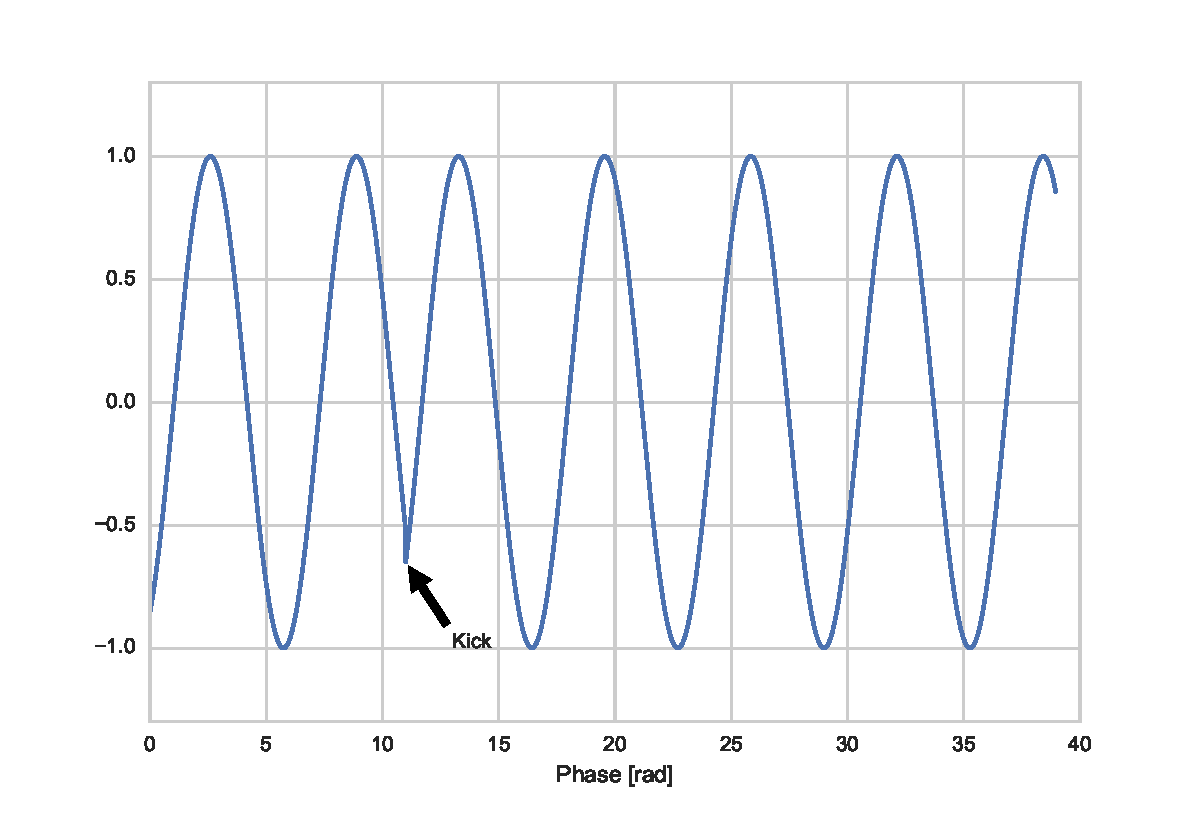
\includegraphics[width=\linewidth]{img/kick}
	\caption{\label{fig:kick}Example of kick in the orbit}
\end{figure}

Two types of perturbations will be described in this section:
\begin{itemize}
	\item static perturbations, which can be  for instance a malfunctioning magnet,
	\item harmonic perturbations, i.e. a perturbation at a given frequency, which can be for instance the \SI{50}{Hz} magnetic field of the main power or the \SI{10}{Hz} field due to a bad isolated power supply.
\end{itemize}

\section{Static perturbation}
\label{sec:loc_static}

\subsection{Theoretical setting of the problem}
The problem is described with the betatron phase variable
\begin{equation}
\Psi = \int\limits_{0}^s \frac{d\sigma}{\beta(\sigma)}.
\end{equation}

The spatial variable $s$ is only used to have a connection between the result and the actual ring. The explanation will be led in the horizontal plane (with the $x$ variable), but is also valid in the vertical one ($y$).

Let one kick be at a given phase $\Psi = \hat{\Psi}$. The orbit is modified and oscillates with a constant period of \SI{2 \pi}{\radian}. Because there is \emph{only one} kick and according to the closed orbit condition, the oscillation after the kick will be stable for one revolution. Furthermore, the orbit must be continuous on all points, thus at the kick position too. This is illustrated in \cref{fig:kick}.

Two revolutions are considered, in order to be sure to find one full revolution without kick. Let $\Psi^\mathrm{ext} \in [0, 4 \pi Q]$ be this new phase (\textit{ext} for extended). The phase $\hat\Psi$ where the kick happens is the one so that
\begin{equation}
\exists (b, c) \in \mathbb{R}^2:
\forall \Psi \in [\hat\Psi, \hat\Psi + 2 \pi Q], \quad
x(\Psi) = b \cos(\Psi + c)
\end{equation}
where Q is the tune of the orbit (see \cref{eq:tune}).

This problem has 3 unknowns which should be determined: $\hat\Psi, b, c$.

\subsection{Practical setting}
In order to know the position of the orbit, BPMs are used.

Only $m$ BPMs are distributed around the orbit. The previous variable can thus be described in a vectorial form
\begin{align}
\begin{cases}
\vec{\Psi} = [\Psi_0, \Psi_1, ..., \Psi_{m-1}] \\
\vec{x} = [x_0, x_1, ..., x_{m-1}]
\end{cases} \quad \mathrm{and} \quad
\begin{cases}
\vec{\Psi}^\mathrm{ext} = [\vec{\Psi}, \vec{\Psi}+2\pi Q ]\\
\vec{x}^\mathrm{ext} = [\vec{x}, \vec{x}]
\end{cases}
\end{align}

\subsection{Solving the problem}

The problem is solved in two steps: first the sine that fits at best the orbit is determined, and second the position of the kick verifying the closed orbit condition (or continuity condition) is found.

An algorithm is designed to find a sine over a revolution, beginning at each BPM and keep the one that fits at best:
\begin{align}
\forall~k \in \, [0,m-1]&, \nonumber \\
&\begin{cases}
\vec{\Psi}^k = \left[\Psi^\mathrm{ext}_{k}, \Psi^\mathrm{ext}_{k+1}, \cdots,  \Psi^\mathrm{ext}_{k+m-1}\right]\\
\vec{x}^k = \left[x^\mathrm{ext}_{k}, x^\mathrm{ext}_{k+1}, \cdots,  x^\mathrm{ext}_{k+m-1}\right]\\
\tilde{\vec{x}} = \mathtt{fit\_sine}\left(\vec{x}^k, \vec{\Psi}^k\right)
\end{cases}
\end{align}

It is then defined
\begin{equation}
k_0 = \underset{k \in [0, m-1]}{\textrm{argmin}}\{||\tilde{\vec{x}}-\vec{x}^k||_2\}
\end{equation}

If there where no noise in the signal, and if the number $m$ of BPMs was infinite, then the kick would be exactly at $\Psi_{k_0}$. However in the real case (with noise), it can only be said that the kick is around $\Psi_{k_0}$, and the closest sine is $\tilde{x}(\Psi) = b \sin(\Psi + c)$.

To find the exact position of the kick, the property of closed orbit is used: the orbit must be continuous also at the kick phase, which means that $\hat{\Psi}$ is the solution of
\begin{align}
b \cos(\Psi + c) &= b\cos(\Psi+c+2 \pi Q),\\
& \mathrm{with}~ \Psi \in [\Psi_{k_0}-A, \Psi_{k_0}+A] , A>0 \nonumber
\end{align}
\begin{align}
&\begin{cases}
\Psi + c &\equiv \Psi + c + 2 \pi Q \pmod{2 \pi} \\
\Psi + c &\equiv - (\Psi + c + 2 \pi Q) \pmod{2 \pi}
\end{cases} \nonumber\\
\iff &\begin{cases}
2 \pi Q &\equiv 0\pmod \pi \qquad\qquad\textit{(Never true)}\\
\Psi &\equiv -c - \pi Q  \pmod \pi
\end{cases} \nonumber
\end{align}

The only possible solutions have the form
\begin{equation}
 \Psi \equiv - c - \pi Q \pmod \pi.
\end{equation}
As the kick is the closest solution to $\Psi_{k_0}$, a constant $K$ is searched so that
\begin{gather}
 -c - \pi Q + K \pi  \leq \Psi_{k_0} \leq -c -\pi Q + (K+1) \pi \nonumber \\
\iff \frac{\Psi_{k_0} + c}{\pi} + Q \leq K \leq \frac{\Psi_{k_0} + c}{\pi} + Q + 1 \nonumber \\
\iff K = \left\lfloor  \frac{\Psi_{k_0}+c}{\pi} + Q \right\rfloor 
\end{gather}
and the two remaining possible values are
\begin{equation}
\left\lbrace - c - \pi Q+ K \pi , \quad - c - \pi Q + (K+1) \pi\right\rbrace
\end{equation}
the kick being chosen as the closest one from $\Psi_{k_0}$.

\subsection{Finding the good sinusoidal}
Several methods are possible to find the best matching sine, for example by using:
\begin{itemize}
	\item a pseudo-inversion
	\item a scalar-product with a sine (resp. a cosine)
\end{itemize}

\paragraph{Pseudo-inversion}
The problem can be set as a linear equation problem as follow.
\begin{align}
&\forall k \in [0,m-1], \tilde{x}(\Psi_k) = a_1 \cos(\Psi_k) + a_2 \sin(\Psi_k) + a \nonumber \\
%
\implies &
\begin{pmatrix}
1 & \cos(\Psi_0) & \sin(\Psi_0) \\
1 & \cos(\Psi_1) & \sin(\Psi_1) \\
\vdots & \vdots & \vdots \\
1 & \cos(\Psi_{m-1}) & \sin(\Psi_{m-1}) \\
\end{pmatrix}
\begin{pmatrix}
a \\ a_1 \\ a_2
\end{pmatrix}
=
\begin{pmatrix}
x_0 \\ x_2 \\ \vdots \\ x_{m-1}
\end{pmatrix} \nonumber
\\
%
\implies &
\begin{pmatrix}
a \\ a_1 \\ a_2
\end{pmatrix}
=
\mathrm{pseudo\_inv}
\begin{pmatrix}
1 & \cos(\Psi_0) & \sin(\Psi_0) \\
1 & \cos(\Psi_1) & \sin(\Psi_1) \\
\vdots & \vdots & \vdots \\
1 & \cos(\Psi_{m-1}) & \sin(\Psi_{m-1}) \\
\end{pmatrix}
\begin{pmatrix}
x_0 \\ x_2 \\ \vdots \\ x_{m-1}
\end{pmatrix}
\end{align}

The pseudo inverse is calculated in \texttt{Matlab} with
\begin{verbatim}
        a = M\x
\end{verbatim}
and in \texttt{Python} with the least-squares method
\begin{verbatim}
        a = numpy.linalg.lstsq(M, x).
\end{verbatim}

\paragraph{Projection on cosine/sine planes}
Since the orbit is expected to be written as
\begin{equation*}
x(\Psi) = a+ a_1 \cos(\Psi) + a_2 \sin(\Psi)
\end{equation*}
it can also be described as
\begin{equation}
x(\Psi) = \scal{x}{1} + \scal{x}{\cos} \cos(\Psi) + \scal{x}{\sin} \sin(\Psi)
\end{equation}
with $\scal{f}{g}$ being the scalar product for real functions: $\int_T f(t)g(t)dt$.

In the numerical case, the scalar product is approximated by its vectorial counterpart by
\begin{align*}
\scal{\vec{f}}{\vec{g}}: \quad
 &\mathcal{R}^n \times \mathcal{R}^n \longrightarrow \mathcal{R} \\
 & (\vec{f},\vec{g}) \quad\longmapsto \quad \frac{1}{n}\sum\limits_{k=0}^{n-1} f_i g_i
\end{align*}

This however provides less good results, as $\sin(\Psi)$ and $\cos(\Psi)$ are numerically orthogonal only if the frequency is a multiple of the sampling frequency divided by the number of samples ($F_s/N$) which cannot be always verified.

\paragraph{Coefficient format}
By defining $b = \sqrt{a_1^2+a_2^2}$ and $c = -\mathrm{arg}(a_1 + j a_2)$ the previous formulas can be written
\begin{equation*}
\tilde{x}(\Psi) = a + a_1 \cos(\Psi) + a_2 \sin(\Psi) = a + b \sin(\Psi + c).
\end{equation*}

\section{Localizing multiple sources}
A step further would be to localize several sources. To do this, one must be able to describe the orbit as an arbitrary piecewise sinusoid function, which is equivalent to the following requirements:
\begin{enumerate}
    \item Find the number of perturbation sources (or piece junctions)
    \item Find the position of theses perturbation sources (or where the junctions are)
\end{enumerate}

The only work in this direction resulted in a brute-force algorithm which would test every single possibility and finally keep the one with the lowest RMS. Further mathematical and algorithmic literature must be studied before deepening this idea.

\section{Harmonic perturbations}
\label{sec:loc_dyn}
Some perturbations can be purely harmonic. The example of the \SI{50}{\hertz} field generated by the main power is an obvious one that cannot be easily isolated. 

As shown in \cref{fig:compare_fofb}, the correction leaves some spikes in the spectrum, which is to be avoided. Hopefully some of them might be localized and removed or isolated, dealing again with the cause of the perturbation instead of its symptom.

Because the storage ring is considered in a first approximation as a linear system, the source of an harmonic perturbation can be localized as an harmonic disturbance with the same frequency. The very same algorithm can thus be used on a pseudo-orbit extracted from the harmonic of interest. 

The harmonic orbit is calculated the same way as in \cref{sec:dyn_corr}, \cref{eq:orbit_extract}, providing a complex vector $\Delta\vec{X}_f$.

If the perturbation is unique, then it is expected to be writable as $d(t) = A_d\cos(2\pi f t + \phi)$ and, because the phase shift is the same for all BPMs, the orbit time signal for the $i$th BPM as 
\begin{equation}
	x_i(t) = \hat{X}_{f,i} \cos (2\pi f t), \qquad \hat{X}_{f,i} \in \mathbb{R}.
\end{equation}
All complex amplitude must thus exactly describe the same sinusoid of frequency $f$ and phase $\alpha_0$, only the amplitude being different at each BPM.
The complex vector $\Delta\vec{X}_f$ can thus be fully described by their amplitudes.

However, since the signal contains also noise and that the perturbation \emph{might} not be unique, it is rotated until the vector of sine (or imaginary part) is minimal, or zero in a ideal case.
\begin{equation}
\begin{cases}\alpha_0 = \underset{\alpha \in [0, 2\pi[}{\textrm{argmin}}\{\Imag{\Delta\vec{X}_f \cdot e^{-j\alpha}} \} \label{eq:harm_perturb_opt}\\
\vec{\hat{X}}_f = \Real {\Delta\vec{X}_f \cdot e^{-j\alpha_0}}
\end{cases}
\end{equation}

This way only one perturbation is considered: the one which contributes the most to the signal.

The new signal $\vec{\hat{X}}_f$ can be used as an differential orbit signal. The kick position is then calculated it with the method described in the static case, \cref{sec:loc_static}.

\remark To achieve the phase optimization given in \cref{eq:harm_perturb_opt}, the Karhunen–Loève transform (or principal component analysis) can be used~\cite{book:wang_2012}. A description of the algorithm is given in \cref{apx:KLT}. If the results are exactly the same, this allows the problem to be solved within a broader theoretical setting. The goal is not anymore to see the sine part vanish but to deal with the perturbation space in which the distortion is the largest. In theory, dealing with each principal component would allow to find the position of each perturbation source.

\section{Experimental results}
\subsection{Artificial static perturbation}
The localization algorithm described above is used on an artificial experiment. All correctors are set to 0, except one which is randomly chosen and given an arbitrary amplitude. The orbit is generated by using the response matrix (see \cref{sec:response_matrix}) and is represented by the green curve on \cref{fig:loc_orbit} (in blue is the final localization).

\begin{figure}
    \centering
    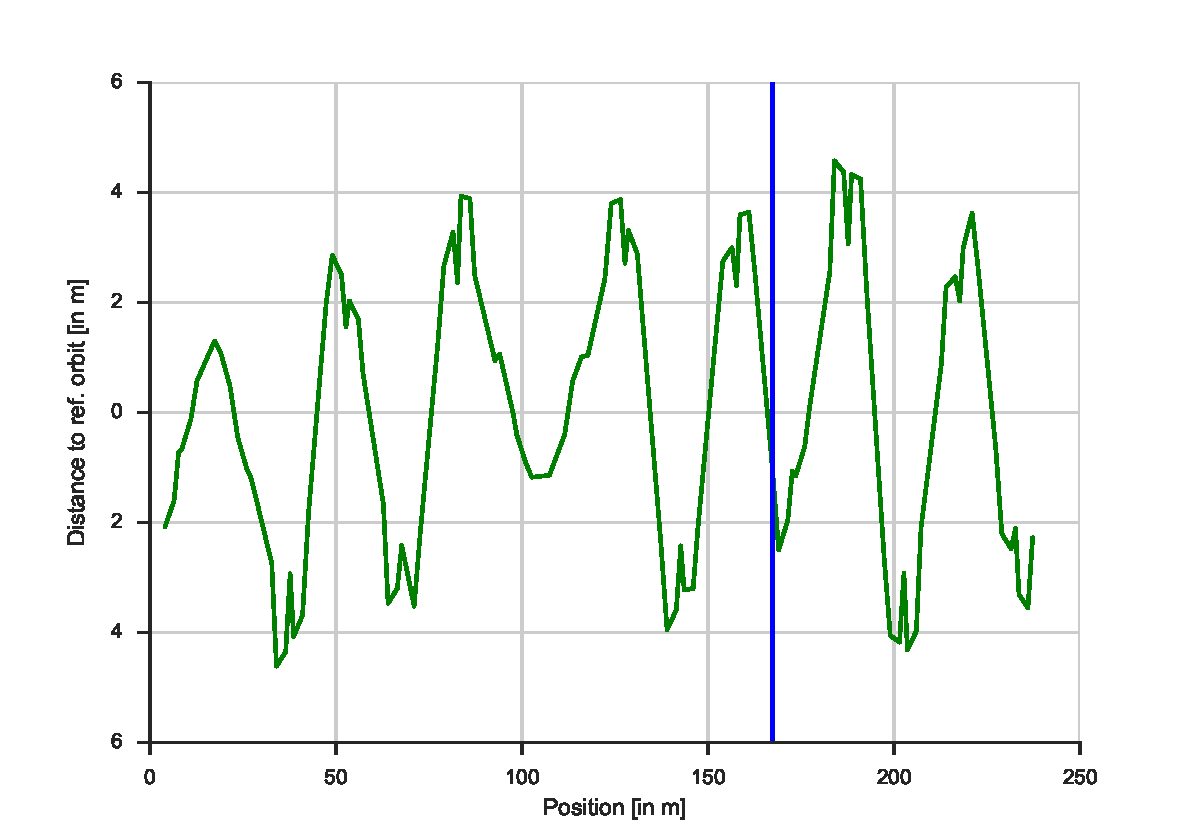
\includegraphics[width=\linewidth]{img/loc_orbit}
    \caption{\label{fig:loc_orbit} Orbit with unique static perturbation}
\end{figure}

The localization algorithm iterations are shown in \cref{fig:loc_errorplots}. The top graph presents in blue the RMS errors between the orbit and a generated sine while setting the kick at each BPM. In green and red are respectively the best fitting amplitudes and phases for each iteration. The convergence is visible and verifies that there are very few risk of being far from the position of the perturbation. However the region where the RMS reaches its smallest value is very flat and thus not very precise.

\begin{figure}
    \centering
    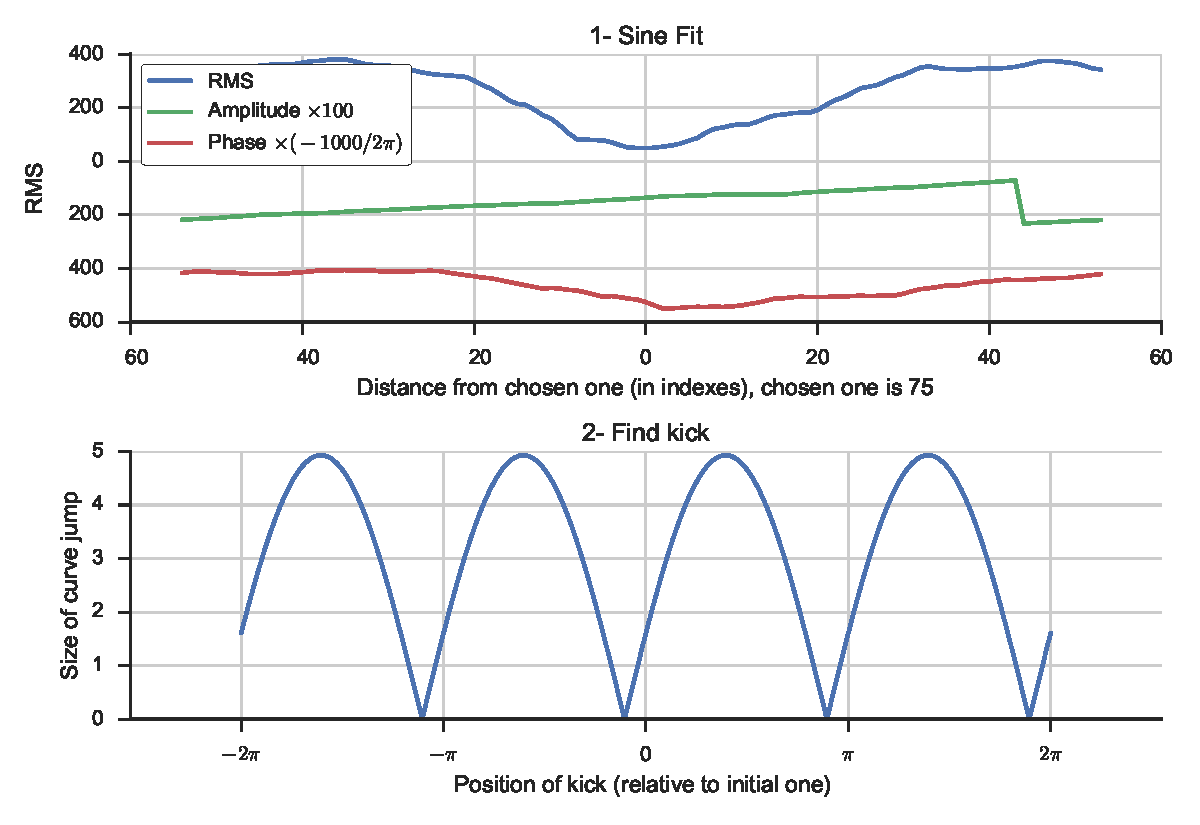
\includegraphics[width=\linewidth]{img/loc_errorplots}
    \caption{\label{fig:loc_errorplots} Error (RMS) and parameters curve of the localization algorithm}
\end{figure}

What is worth remarking is that the amplitude and phase vary quite continually, meaning that choosing the wrong position to set the sinus parameters is not too harmful. This validates the idea of first setting the sinusoid parameters and then find the exact position of the kick.

On the second graph (\cref{fig:loc_errorplots}, below) is represented the jump done by the curve left and right from the BPM chosen to set the sinusoid parameters. In the algorithm, the first minimum of the curve is defined as the kick position.

Finally the orbit and the sinusoid constructed by the algorithm can be seen on \cref{fig:loc_reconstructed_sine}. They are quite overlapping and the closed orbit condition is verified.

\begin{figure}
    \centering
    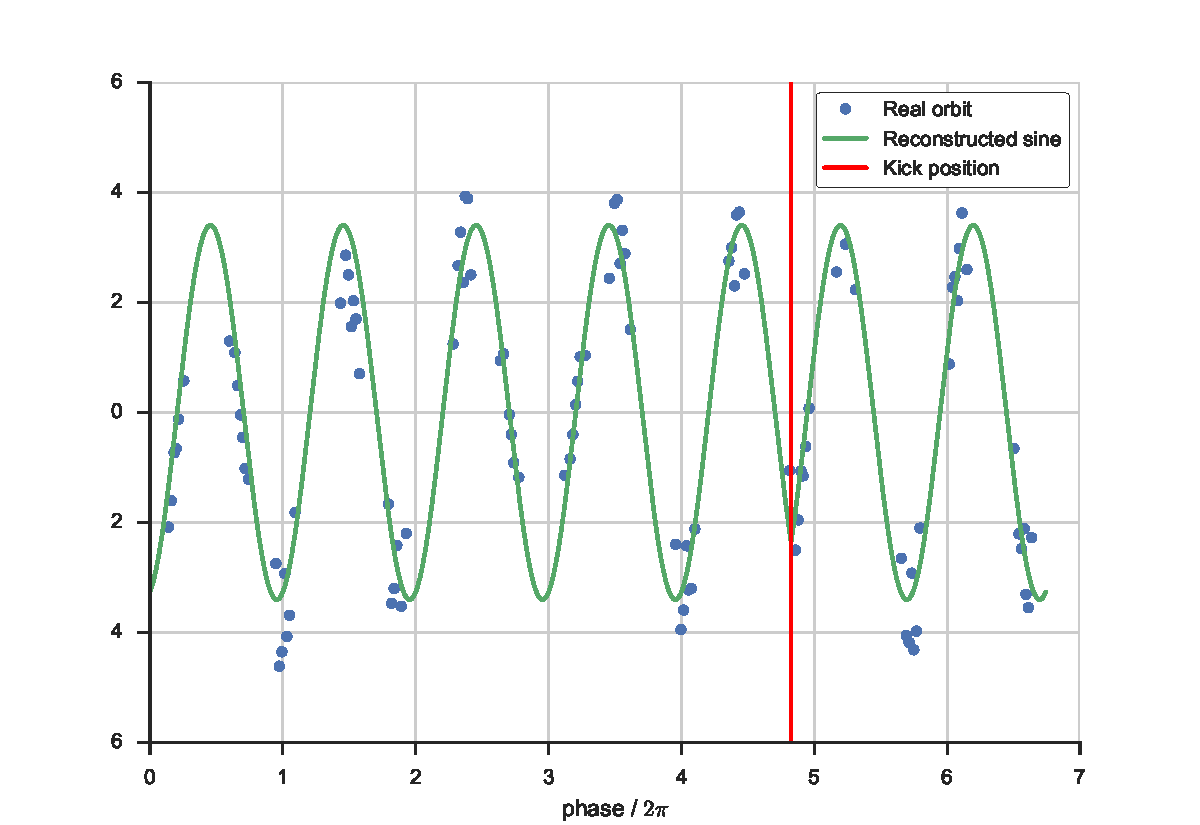
\includegraphics[width=\linewidth]{img/loc_reconstructed_sine}
    \caption{\label{fig:loc_reconstructed_sine} Reconstructed sinusoid and orbit}
\end{figure}

\begin{figure}
	\centering
	\begin{subfigure}[b]{\textwidth}
		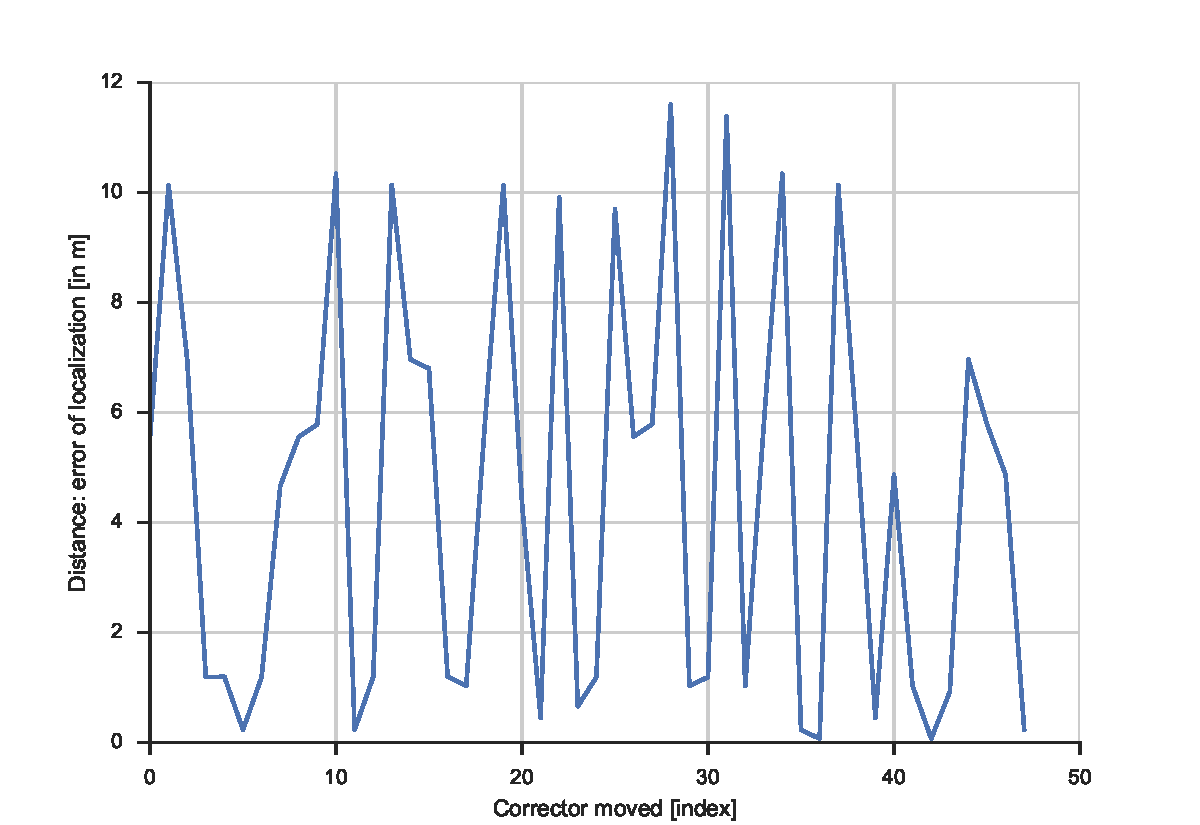
\includegraphics[width=\linewidth]{img/loc_all_x}
		\caption{Horizontal}
	\end{subfigure}
	\begin{subfigure}[b]{\textwidth}
		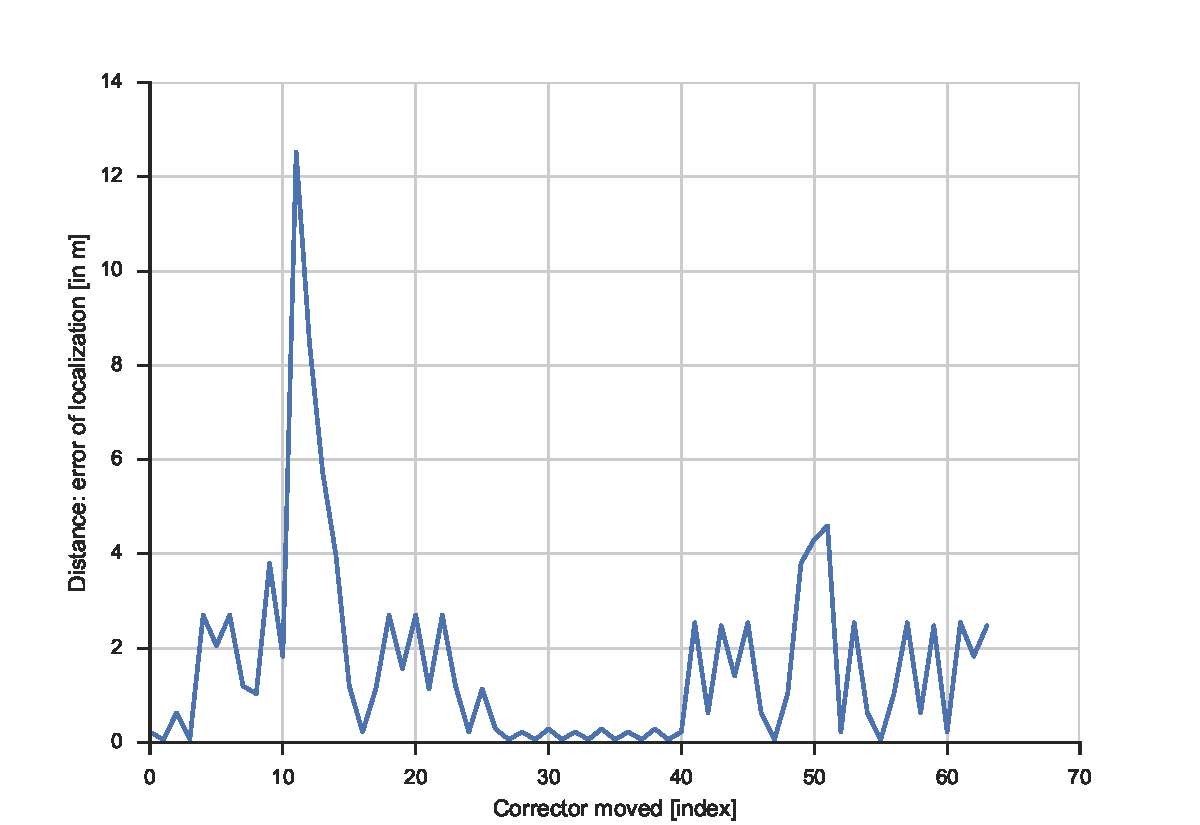
\includegraphics[width=\linewidth]{img/loc_all_y}
		\caption{Vertical}
	\end{subfigure}
	\caption{\label{fig:loc_all_corr} Localization error for all correctors}
\end{figure}

The same artificial experiment was conducted by setting each corrector separately to an arbitrary value and trying to localize it back. \Cref{fig:loc_all_corr} shows the localization errors. It appears that the localization error in such an environment is quite precise in the vertical direction ($d \approx \SI{2}{\meter}$ on a ring of \SI{240}{\meter}), except around the 11th corrector. In this area, during the measurement of the response matrix used to generate the artificial orbit was activated a 7 Tesla wiggler, which is a device for producing intense X-rays from the electron beam; this means that it has a significant impact on the orbit optics and is therefore likely to degrade the localization process. A real test, directly on the storage ring, would certainly provide better results at this position, but reduce the overall precision because of measurement noises. In the horizontal direction, the results are less accurate because the number of available points by oscillation is lower. The horizontal tune is approximatively 17.85 whereas the vertical one is 6.74, while the number of BPMs is identical in both directions.

Even by taking the worst localization error, it reduces the source position to less than $1/10$ of the orbit circumference, which is already a non-negligible gain in the perturbation source removal process.

\subsection{10 Hertz harmonic perturbation}
A similar simulation was conducted for the harmonic simulation. Instead of setting the selected corrector magnet to an arbitrary amplitude, it is set to a sine with an arbitrary phase (in this case, random between 0 and $\SI{2\pi}{\radian}$), sampled at $F_s=\SI{150}{\hertz}$. Every sample vector is then multiplied with the response matrix, which results in an orbit sample. This orbit can then be used as the input of the algorithm presented in \cref{sec:loc_dyn}.

The localization results are exactly the same as in the static case, provided that enough samples are used (for example, \SI{10}{\second} at \SI{150}{\hertz}, for frequencies up to \SI{70}{\hertz}) and that the added noise is not too high.

\section{Summary}
Instead of trying to correct some perturbations, isolating or removing their source would be very appealing. With the described algorithms, one can expect to reduce the potential zone to up to \SI{2}{\meter} (which is less than 1\% of the ring circumference) in perfect conditions, and in the worst case around 10 to \SI{20}{\meter} (or around 10\% of the circumference). With such a reduced area, it is very conceivable to determine the actual source, either with a mobile magnetometer or simply by observing the suspicious devices.
